\section{Components and Application Responsibilities}
The framework separates application handlers from the machinery that discovers Providers, correlates messages, and checks invocation state. A ServiceUser manages outgoing requests and their callbacks. A ServiceProvider registers service handlers and processes selected invocations. A ServiceController manages permissions and authorization material. These are software roles: a ground station can consume camera services while providing image analysis, and a compute node can request an upstream service while executing its own assigned work.

\begin{figure}[htbp]\singlespacing\centering
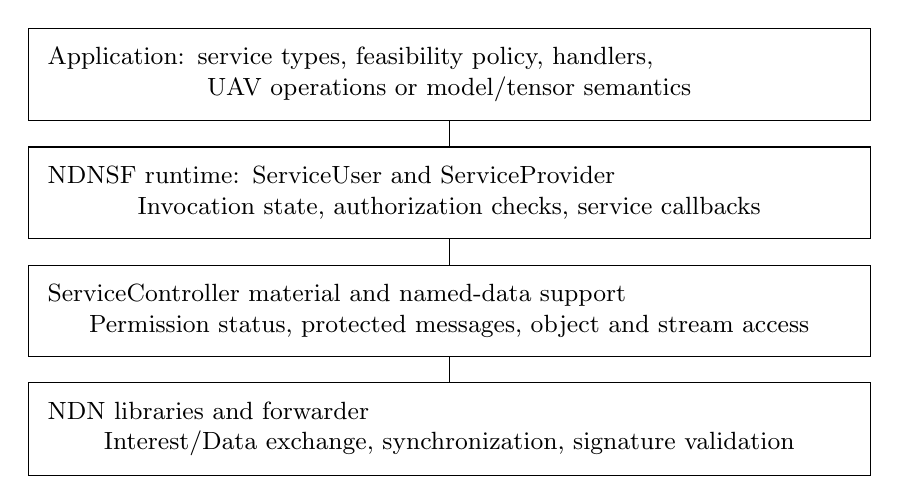
\begin{tikzpicture}[every node/.style={draw,align=center,font=\small,text width=10.2cm,inner sep=7pt}]
\node (app) at (0,0) {Application: service types, feasibility policy, handlers,\newline UAV operations or model/tensor semantics};
\node (runtime) at (0,-1.5) {NDNSF runtime: ServiceUser and ServiceProvider\newline Invocation state, authorization checks, service callbacks};
\node (authority) at (0,-3) {ServiceController material and named-data support\newline Permission status, protected messages, object and stream access};
\node (ndn) at (0,-4.5) {NDN libraries and forwarder\newline Interest/Data exchange, synchronization, signature validation};
\draw (app)--(runtime);\draw (runtime)--(authority);\draw (authority)--(ndn);
\end{tikzpicture}
\caption{Responsibility groups in the framework. Lines denote software dependencies, not packet directions or a mandatory deployment topology. The Controller is a logical authority, not an on-path relay for every exchange.}
\end{figure}

Application code defines the meaning of a service and supplies its feasibility and execution logic. The framework cannot determine from a valid ACK whether a camera truly has an unobstructed view or whether an advertised GPU can meet a prediction deadline. It can associate the ACK with the request, verify the participating identity and required protected values, and apply the configured selection policy. A positive ACK expresses willingness subject to the request's conditions; it is not evidence that execution has finished or a reservation unless the protocol explicitly provides one.

The ServiceContainer supports composition of runtime roles and local services within a process. Its local registry gives trusted components a way to invoke registered application functionality without turning every internal call into a network exchange. The application must keep the runtime and callback dependencies alive until active operations are closed. Local composition is useful for shared camera or inference facilities, but remote callers cannot select it as an alternative authorization path.

The current typed C++ interface illustrates this separation. The following shortened example uses application-defined, serializable status messages; identity provisioning, event-loop setup, and error handling are omitted. It illustrates application programming interface (API) use rather than a standalone executable.
\begin{lstlisting}[language=C++,caption={Typed registration and invocation of a compact status service.}]
provider.addHandler<StatusQuery, StatusReply>(
  ndn::Name("/status"),
  [](const ndn::Name& requester,
     const StatusQuery& query, StatusReply& reply) {
    readApplicationStatus(query, reply);
  });

user.RequestService<StatusQuery, StatusReply>(
  candidates, ndn::Name("/status"), query,
  [](const StatusReply& reply) { displayStatus(reply); },
  []() { reportTimeout(); }, 2000);
\end{lstlisting}

The handler interprets the query and fills the reply. The User interface supplies an invocation timeout and result callbacks, while NDNSF manages the surrounding exchange. A service requiring confidential execution input uses the protected input-delivery path described below; this compact example does not prescribe placing arbitrary application input in discovery. Typed serialization removes some repeated application glue, but does not establish semantic compatibility between different service versions. That remains part of the service contract.
